\documentclass{CUP-JNL-DTM}%


%%%% Packages
\usepackage{graphicx}
\usepackage{multicol,multirow}
\usepackage{amsmath,amssymb,amsfonts}
\usepackage{mathrsfs}
\usepackage{amsthm}
\usepackage{rotating}
\usepackage{appendix}
% For JDM please remove the natbib package:
\usepackage[numbers]{natbib}
% And use biblatex-apa with a .bib file to format your references according to the APA7 style.
% \usepackage[natbib,style=apa]{biblatex}
% \addbibresource{your-refs.bib}
\usepackage{ifpdf}
\usepackage[T1]{fontenc}
\usepackage{newtxtext}
\usepackage{newtxmath}
\usepackage{textcomp}
\usepackage{xcolor}
\usepackage{lipsum}
\usepackage{float}
\usepackage{subcaption}
\usepackage[spanish]{babel}
\usepackage[colorlinks,allcolors=blue]{hyperref}


\newtheorem{theorem}{Theorem}[section]
\newtheorem{lemma}[theorem]{Lemma}
\theoremstyle{definition}
\newtheorem{remark}[theorem]{Remark}
\newtheorem{example}[theorem]{Example}
\numberwithin{equation}{section}


\jname{Universidad San Francisco de Quito}
\articletype{}
\artid{}
\jyear{2025}
\jvol{}
\jissue{}
%\raggedbottom


\begin{document}

\begin{Frontmatter}

\title[Article Title]{High Energy physics project}

% There is no need to include ORCID IDs in your .pdf; this information is captured by the submission portal when a manuscript is submitted. 
\author[1]{Jos\'e David Ochoa Flores}

\authormark{Author Name1 \textit{et al}.}

\address[1]{\orgdiv{Maestr\'ia de F\'isica}, \orgname{Universidad San Francisco de Quito}, \orgaddress{\city{Quito}, \country{Ecuador}}}


\authormark{Jos\'e Ochoa}

\keywords{Simulation, chain, Drell-Yan, Beyond Standard Model, FeynRules}

\abstract{The following project aims to simulate a BSM model using the \textit{FeynRules}}

\end{Frontmatter}

% Some math journals (FLO) require a table of contents. Comment out this line if no ToC is needed.
%\localtableofcontents

\section[Seccion 1]{Seccion 1}


Next we detail the full simulation chain of a Drell-Yan process. 


\begin{figure}[H]
    \FIG{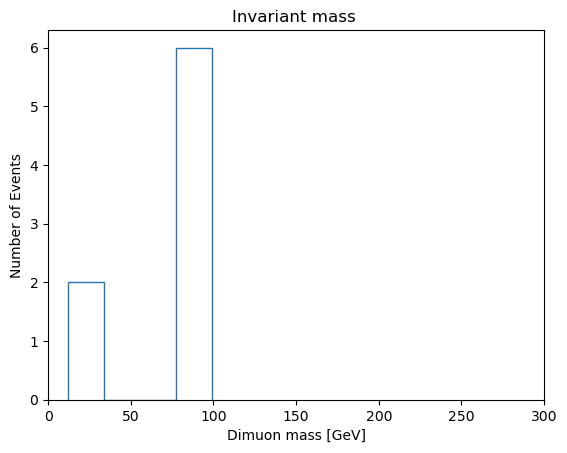
\includegraphics[width=0.5\textwidth]{img/dy_ele_imass.png}}
    {\caption{$J/\psi mass fit$}
    \label{fig1}}
\end{figure}


\begin{figure}[H]
    \begin{subfigure}{.5\textwidth}
      \centering
      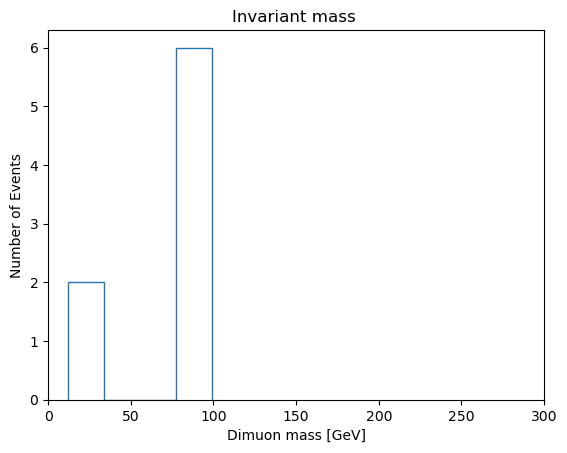
\includegraphics[width=.8\linewidth]{img/dy_ele_imass.png}
      \caption{Trigger efficiency Monte Carlo}
      \label{fig:sfig1}
    \end{subfigure}%
    \begin{subfigure}{.5\textwidth}
      \centering
      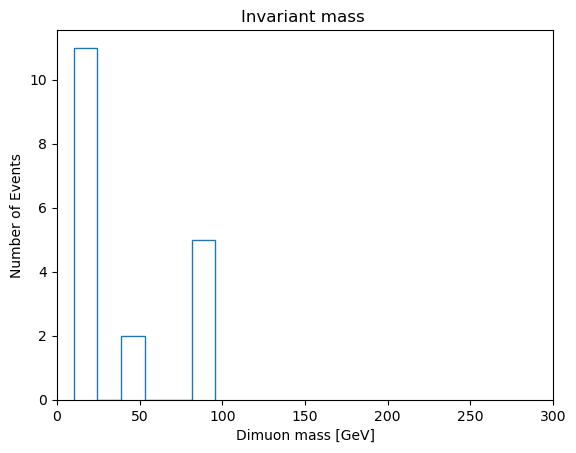
\includegraphics[width=.8\linewidth]{img/dy_muon_imass.png}
      \caption{Trigger efficiency Data}
      \label{fig:sfig2}
    \end{subfigure}
    \caption{Plots for trigger efficiency}
    \label{fig:fig}
\end{figure}

\section{Conclusion}


\begin{Backmatter}
% For JDM please remove this \begin{thebibliography}...\end{thebibliography} list.
% Use biblatex-apa (see instructions in preamble) instead, and write \printbibliography here to print the reference list in APA7 style.
\begin{thebibliography}{}

\end{thebibliography}

\end{Backmatter}

\end{document}
